\documentclass[11pt,twocolumn]{article}

\usepackage{amssymb} \usepackage{graphicx} \graphicspath{ {../imgs/} }

\renewcommand{\thesection}{\Roman{section}}
\renewcommand{\thesubsection}{\thesection.\Roman{subsection}}

\title{Topological Methods in Path Planning} \author{Daniel Bencic}
\date{25.08.2022}

\begin{document}
\maketitle

\section{Introduction} One of the crucial tasks for every autonomous
robot is finding a collision free path through free space. Due to it's
importance this problem has been studied for decades and is know as
the path planning or the ``piano movers'' problem
\cite{schwartzPianoMoversProblem1983a,schwartzPianoMoversProblem1983b}.
Abstract reasoning is a key part of solving complex problems in an
intelligent way \cite{zuckerGroundedTheoryAbstraction2003}. Since
topology studies the properties of spaces, incorporating it into
solving the path planning problem leads to algorithms ``making sense''
of it's solutions.

The review is structured in the following way: Chapter II introduces
basic preliminaries. Chapter III gives an overview of the most
influential path planning methods. Chapter IV is the main part where
we review different methods from topology used in the path planning
problem. Finally Chapter V discusses possible future research
directions.

\section{Problem Formulation}
\subsection*{Preliminaries} This section introduces some fundamental
concepts of topology and path planning
\cite{munkresTopology2014,lavallePlanningAlgorithms2006,hatcherAlgebraicTopology2002}.

\textbf{Homeomorphism} If there exists a bijective function
\(f: X \mapsto Y\) such that \(f\) and it's inverse \(f^{-1}\) are
continuous functions, then the topological spaces \(X\) and \(Y\) are
homeomorphic. Homeomorphism implies that both \(X\) and \(Y\) share
the same topological properties.

\textbf{Configuration Space} Given a metric space \(\mathcal{W}\) with
metric \(d\) and a rigid body \(\mathcal{A}\), a rigid body
transformation is a function \(f: \mathcal{A} \mapsto \mathcal{W}\)
such that \(d(a_{1}, a_{2}) = d(f(a_{1}), f(a_{2}))\) and no
reflection occurs. This holds for rotations and translations. Given
\(GL(n)\) by the set of all invertible \(n \times n\) matrices,
\(O(n)\) is a subgroup of \(GL(n)\) such that \(QQ^{T} = Q^{T}Q = I\)
for all \(Q \in O(n)\). The subgroup \(SO(n)\) of \(O(n)\) which
contains all rotations matrices meaning \(det(P) = 1\) for all
\(P \in SE(n)\). Combining arbitrary rotations and translations gives
the special euclidean group \(SE(n)\) which is homeomorphic to
\(\mathbb{R}^{n} \times SO(n)\).

The configuration space for a rigid robot is therefore
\(\mathcal{C} \cong \mathbb{R}^{2} \times \mathbb{S}^{1}\) and
\(\mathcal{C} \cong \mathbb{R}^{3} \times \mathbb{RP}^{3}\) in 2D
space and 3D space, respectively.

\textbf{Path} Given two points \(x_{0}, x_{1} \in X\), a path is a
continous function \(f: [0, 1] \mapsto X\) such that \(f(0) = x_{0}\)
and \(f(1) = x_{1}\). Paths for which \(f(0) = f(1) = x_{0}\) are
loops with basepoint \(x_{0}\).

\textbf{Homotopy} Two paths \(f\) and \(g\) with the same endpoints
are homotopic if one can be continuously deformed into the
other. Formally, there exists a familiy
\(f_{t}: [0, 1] \mapsto X, 0 \le t \le 1\) such that
\(f_{t}(0) = x_{0}\), \(f_{t}(1) = x_{1}\) and \(f_{0}(s) = f(s)\),
\(f_{1}(s) = g(s)\) and the function
\(F(s, t): [0, 1] \times [0, 1] \mapsto X\) defined by
\(F(s, t) = f_{t}(s)\) is continuous (Figure \ref{fig:homotopy}).

\begin{figure}[h] \centering 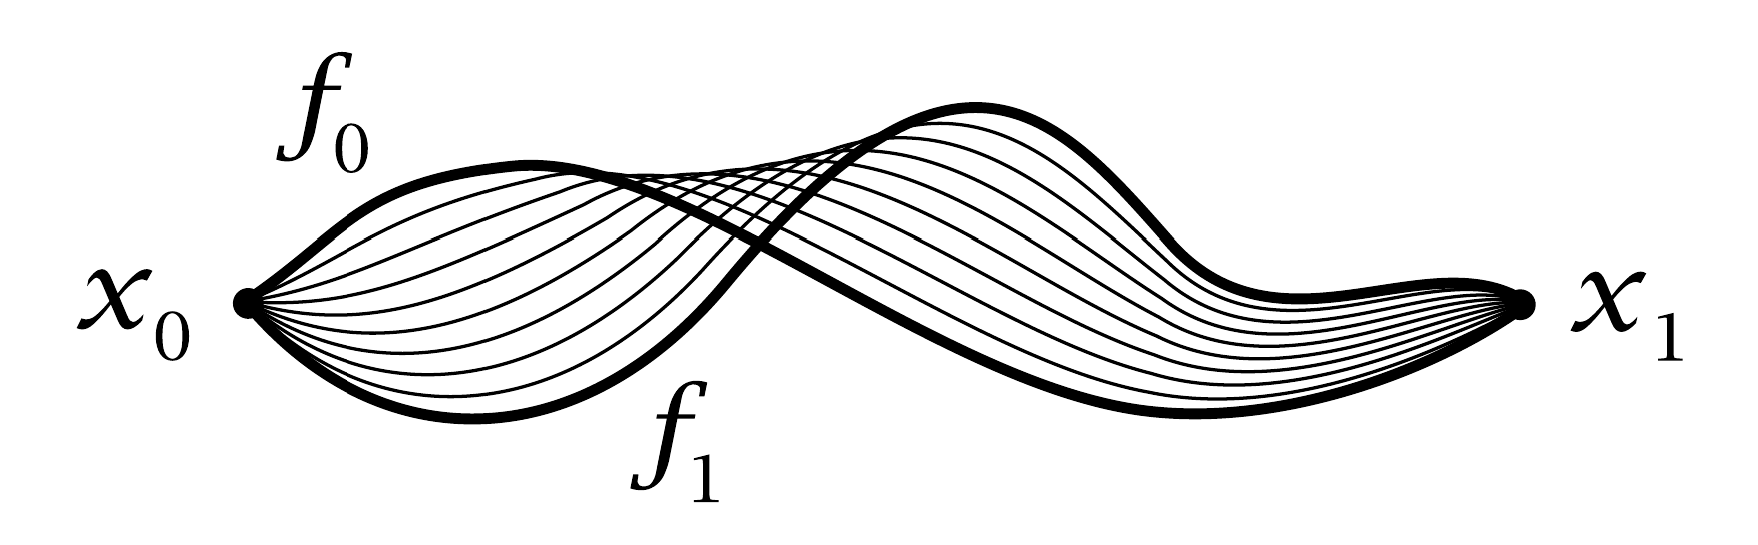
\includegraphics[scale=.18]{homotopy}
  \caption{Homotopy \cite{hatcherAlgebraicTopology2002}.}
  \label{fig:homotopy}
\end{figure}

\textbf{Fiber Bundle} A fiber bundle is a structure on a space \(E\)
with fiber \(F\) and a projection \(p: E \mapsto B\) such that a
homeomorphism \(h: p^{-1}(U) \mapsto U \times F\) exists for a
neighborhood of every point of \(B\). The map \(h\) therefore maps
each fiber \(F_{b} = p^{-1}(b)\) homeomorphically onto the copy
\(\{b\} \times F\) of \(F\). The space \(E\) is called total space and
\(B\) is called the base space of the bundle.

\subsection*{The Path Planning Problem} Given the set of all possible
transformations of a rigid robot \(\mathcal{C}\) and the
transformations that lead to a collision with obstacles
\(\mathcal{C}_{obs}\), the free space is
\(\mathcal{C}_{free} = \mathcal{C} \setminus \mathcal{C}_{obs}\)
(Figure \ref{fig:cspace}). Let \(q_I\) be the initial configuration
and \(q_G\) the goal configuration. The solution to the path planning
problem is a continuous path
\(\pi: [0, 1] \mapsto \mathcal{C}_{free}\) where \(\pi(0) = q_I\) and
\(\pi(1) = q_G\).

\begin{figure}[h] \centering 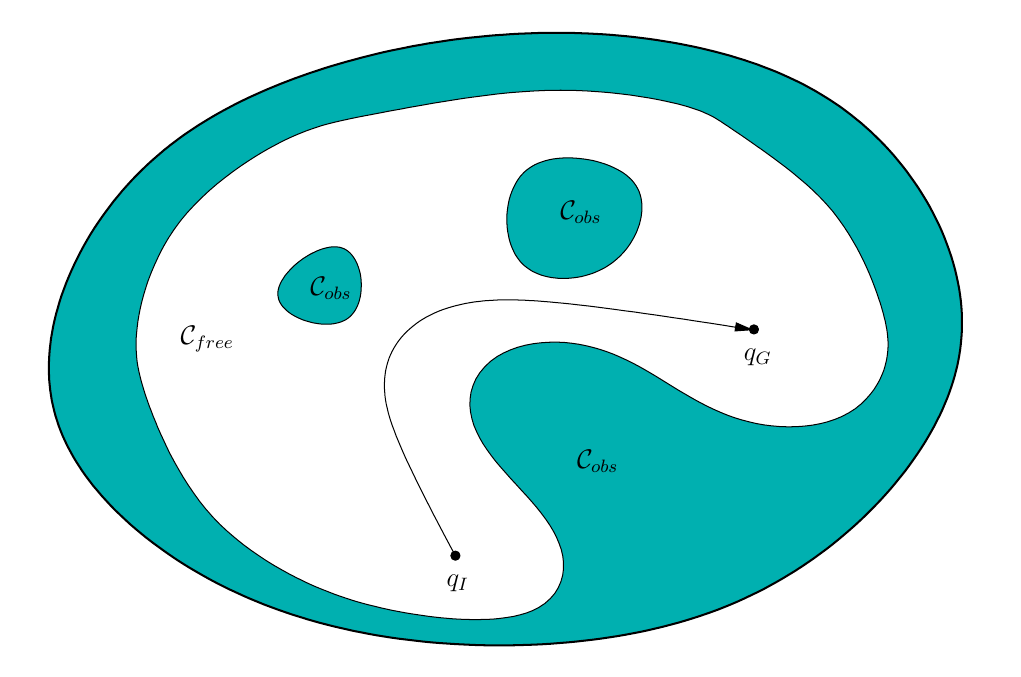
\includegraphics[scale=.25]{cspace}
  \caption{The path planning problem
    \cite{lavallePlanningAlgorithms2006}.}
  \label{fig:cspace}
\end{figure}

\begin{figure}[h] \centering
  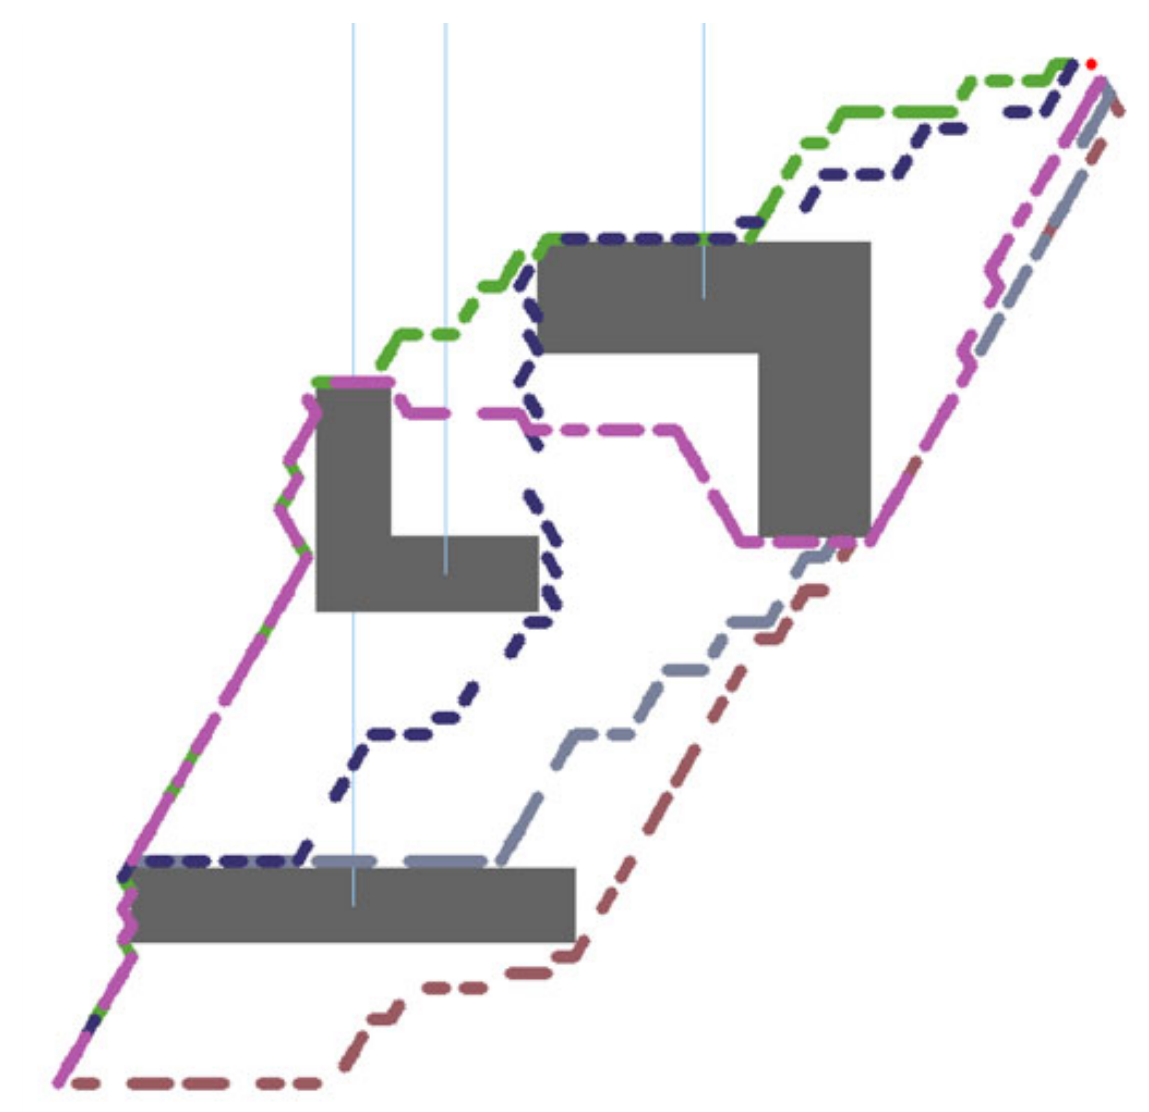
\includegraphics[scale=.2]{homotopy_classes}
  \label{fig:homotopy_classes}
  \caption{Paths belonging to different homotopy classes
    \cite{bhattacharyaPathHomotopyInvariants2018}.}
\end{figure}

\section*{Related Work}
\subsection*{Path Planning} Due to the computational complexity of the
path planning problem, there are different approaches to solve this
problem in polynomial time.

\textbf{Graph search}. These approaches assume that \(\mathcal{C}\) is
in the form of a graph. They then apply graph search techniques to
find the path \(\pi\). A widely used algorithm to compute shortest
paths in a graph is Dijkstra's algorithm
\cite{dijkstraNoteTwoProblems1959}. It is a greedy algorithm that
computes the shortest path from every node to every other node in the
graph. The next node for expansion is selected based on the lowest
cost-to-come \(\hat g(x)\). It is \textit{complete}, meaning it finds
a solution if one exists and reports failure otherwise. It is also
\textit{optimal} in the sense that the computed path is the shortest
possible path.

A* \cite{hartFormalBasisHeuristic1968} improves Dijkstra's algorithm
by reducing the number of expanded nodes in the graph. This is
achieved by using a different function
\(\hat f(x) = \hat g(x) + \hat h(x)\) to select the next node for
expansion. The term \(\hat h(x)\) is a heuristic for the least
possible cost-to-go in a metric space. Many path planning algorithms
in the current literature build upon A* (Figure
\ref{fig:graph-search}).

\begin{figure}[h] \centering
  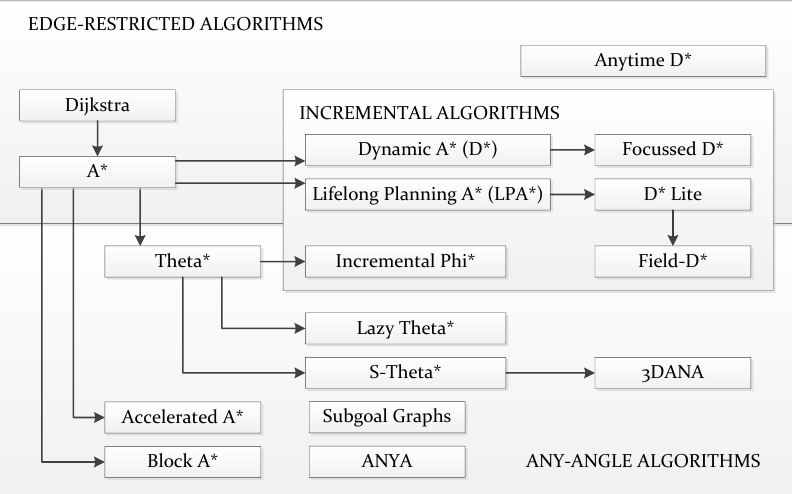
\includegraphics[scale=.35]{graph_search_algorithms}
  \caption{Evolution of graph search algorithms for the path planning
    problem \cite{sanchez-ibanezPathPlanningAutonomous2021}.}
  \label{fig:graph-search}
\end{figure}

Stentz et al. developed D*, an incremental algorithm based on A* that
is able to find shortest paths on maps with changing costs, i.e. due
to a robot moving trough the environment and updating the map. D*
computes a path backwards from the goal to the robot. Koenig et
al. \cite{koenigIncremental2001} also proposed an incremental version
of A* (LPA*), where successive runs only recalculate locally
inconsistent nodes. They combined it with the backward search of D*
and created D*-Lite \cite{koenigLite2002}, a less complex version of
D* with at least the same performance therefore making D* obsolete.

Daniel et al. \cite{danielThetaAnyAnglePath2010} showed an approach
specifically for grid-maps that is not limited to predefined angles
for the transition to other grid cells. It is based on A* and uses
line of sight to determine successor nodes. Another any-angle approach
proposed by Ferguson et al.  \cite{fergusonFieldAlgorithmImproved2005}
uses linear interpolation to find the least cost path trough a cell
and produces globally smooth paths.

A comprehensive review of graph search algorithms for the path
planning problem can be found in the literature
\cite{aitsaadiUAVPathPlanning2022,sanchez-ibanezPathPlanningAutonomous2021,yanComprehensiveSurveyAnalysis2020,nashAnyAnglePathPlanning2013}.

\textbf{Sampling}. Due to the curse of dimensionality
\cite{bellmanDynamicProgramming1984}, graph search in high dimensional
configuration spaces can quickly become computationally intractable.
Sampling-based approaches discretize the high-dimensional
configuration space by generating random samples in
\(\mathcal{C}_{free}\). One highly influential contribution from
Kavraki et. al. \cite{kavrakiProbabilisticRoadmapsPath1996} is called
Probabilistic Roadmap Method (PRM). It is a solution to the
multi-query path planning problem in high dimensional configuration
spaces. The method consists of a learning and a query phase. The
former repeatedly generates a random configuration in
\(\mathcal{C}_{free}\) and connects this sample to neighboring nodes
in a given radius with a fast local planner. In addition, a heuristic
is used to generate extra nodes in ``difficult'' regions of
\(\mathcal{C}_{free}\). The method is therefore influenced by the
topological properties of \(\mathcal{C}_{free}\). The result is a
graph representation of \(\mathcal{C}_{free}\) in the form of a forest
of trees.

Another highly cited approach using only a single tree is the
Rapidly-exploring Random Tree (RRT) algorithm by Lavalle
\cite{lavalleRapidlyExploringRandomTrees1998}. The algorithm grows a
tree in \(\mathcal{C}_{free}\) by generating a sample from a uniform
distribution and growing the nearest node of the tree in the direction
of the sample. Since the probability that a node is selected for
expansion is proportional to the size of it's Voronoi cell (see Figure
\ref{fig:rrt}), the tree grows with a bias towards unexplored regions
in \(\mathcal{C}_{free}\).

\begin{figure}[h] \centering 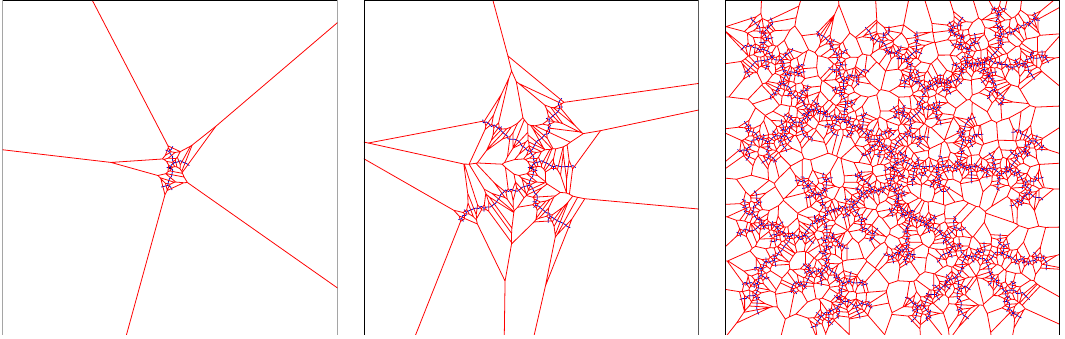
\includegraphics[scale=.275]{rrt_voronoi}
  \caption{Voronoi diagram of a RRT tree.}
  \label{fig:rrt}
\end{figure}

Karaman et. al. \cite{karamanSamplingbasedAlgorithmsOptimal2011}
showed that both PRM and RRT algorithms are not asymptotically
optimal. That means that with a growing number of nodes the
probability that the algorithm finds an optimal solution converges to
zero. In their paper they also proposed two new algorithms PRM* and
RRT* which are shown to be asymptotically optimal. The former was
improved by calculating the radius, in which a sample is connected to
it's neighbors, based on the number of present samples. The latter was
improved by selecting the node for expansion based on the cost-to-come
in the neighborhood of a sample and rewiring the tree after insertion
of a new node.

There are many algorithms improving and extending RRT and RRT* in the
literature. With RRT-Connect, Kuffner et. al.
\cite{kuffnerRRTConnectEfficientApproach} introduced a bidirectional
RRT that grows one tree from \(q_I\) and another tree from \(q_G\)
while trying to connect the two trees. Anytime RRT*
\cite{karamanAnytimeMotionPlanning2011} returns a fast initial
solution and a robot commits to execute a subset of the full path
\(\pi_{com}: [0, t_{com}] \mapsto C_{free}\). While executing
\(\pi_{com}\) the remaining path is further improved until the robot
commits to the next subset of the path. Realizing that there is a
subset of \(C_{free}\) that contains configurations that are
guaranteed to improve the current solution, Informed RRT*
\cite{gammellInformedRRTOptimal2014} uses a ellipsoidal heuristic to
sample from this set and improve the convergence rate of RRT*. BIT*
\cite{gammellBatchInformedTrees2015} does not sample a single
configuration, instead it samples a batch of configurations and grows
a tree from this batch.  After finding a solution or no further
possible expansion, the next batch is sampled. If a solution has been
found with the previous batch, this batch is sampled from the
ellipsoidal subset introduced by Informed RRT* and the tree is updated
by identifying locally inconsistent nodes.

A comprehensive review of RRT* variants has been published by Noreen
et. al.  \cite{noreenOptimalPathPlanning2016a} and a review of more
sampling-based approaches for the path planning problem can be found
in \cite{elbanhawiSamplingBasedRobotMotion2014}.

\subsection*{Topological Methods}
\subsubsection*{Homotopy Invariants}
Given a map that associates to every path the pair of start and
endpoints \(\pi: PX \mapsto X \times Y\), Farber
et. al. \cite{farberTopologicalComplexityMotion2003} define the motion
planning problem as finding a function \(s: X \times X \mapsto PX\)
such that \(\pi \circ s = id\). They introduce
the notion of continuous motion planning, where close initial-final
pairs produce close paths. Based on this definition, they introduce a
homotopy invariant called topological complexity (\(\textbf{TC}(X)\))
which is the minimal number \(k\) such that
\[X \times X = U_{1} \cup U_{2} \cup ... \cup U_{k}\]
and there exists a continuous motion planning for each \(U_{i}\).

Bhattachary
et. al. \cite{bhattacharyaSearchbasedPathPlanning2010,bhattacharyaSearchBasedPathPlanning2012}
construct an augmented graph that can then be searched with classic
graph search algorithms. Given a graph \(G = (V, E)\), the augmented
graph is a lift of \(G\) into the covering space of \(X\). In
configuration spaces homeomorphic to \(\mathbb{R}^{2}\) they use
Cauchy's Integral Theorem and the Residue Theorem from complex
analysis to calculate a \(L\)-value which is equal for paths in the
same homtopy classes and not equal otherwise. In configuration spaces
homeomorphic to \(\mathbb{R}^{3}\) they use laws from electromagnetism
to calculate a \(H\)-value. These values are then used to augment the
respective graphs.  They propose another method to augment a graph in
\cite{bhattacharyaPathHomotopyInvariants2018}.  Here homotopy
invariants for a \(D\)-dimensional manifold \(X\) are constructed by
introducing \((D - 1)\)-submanifolds. Words are then formed by tracing
a path \(f\) and inserting a letter every time \(f\) intersects one of
the submanifolds.

\begin{figure}[h] \centering
  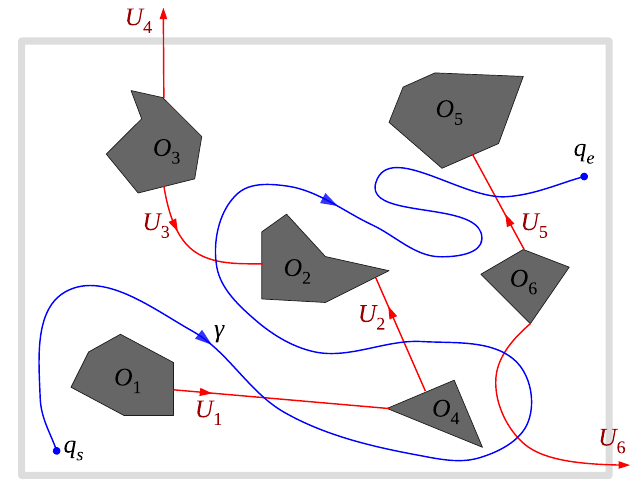
\includegraphics[scale=.4]{word_construction}
  \caption{The blue path yields the constructed word
    \(h(\gamma) = u_{1}^{-1} u_{6} u_{6}^{-1} u_{2} u_{3} u_{5}^{-1} =
    u_{1} u_{2} u_{3} u_{5}^{-1}\)
    \cite{bhattacharyaPathHomotopyInvariants2018}.}
  \label{fig:word-construction}
\end{figure}

While Bhattachary et. al. proposed a homotopy invariant for graph
search, Sakcak et. al. \cite{sakcakHomotopyAwareKinodynamic2019}
propose a homotopy invariant for the use with kinodynamic path
planning with RRT-based planners. ...

In \cite{bhattacharyaPersistentHomologyPath2015} the authors try to
solve the problem of how to threshold an occupancy grid map to get a
binary map for the use with classic path planning techniques. They use
persistent homology to get the homology class of paths that is
persistent over the widest range of threshold values.

Wang et. al. \cite{wangConstructingFinerThen2022} show a method for
constructing path classes in the workspace which are finder but extend
to homotopy classes in the configuration space. °°Fiberbundle°°

Yang et. al. \cite{yangEfficientSearchShortest2022} propose a method
to calculate the \(k\)-shortest non-homotopic paths by simplifiying
the topology and discarding \(2^{n} - k\) of the \(2^{n}\) possible
paths in a two dimensional environment with \(n\) obstacles.

Liang et. al. \cite{liangHomotopyDrivenExplorationHumanmade2021}
developed an algorithm for a robot to explore human-made space
autonomously. Signs are used to dictate the general direction and if
this direction is a dead end, backtracking is performed and a
different homotopy class is explored.

An approach for exploration with a tethered robot is proposed by the
authors of \cite{shapovalovExplorationUnknownEnvironments2020} . They
use homotopy information to limit the length of the tether and ensure
that entanglement of the tether is avoided (see Figure
\ref{fig:tethered-exploration}).

\begin{figure}[h] \centering
  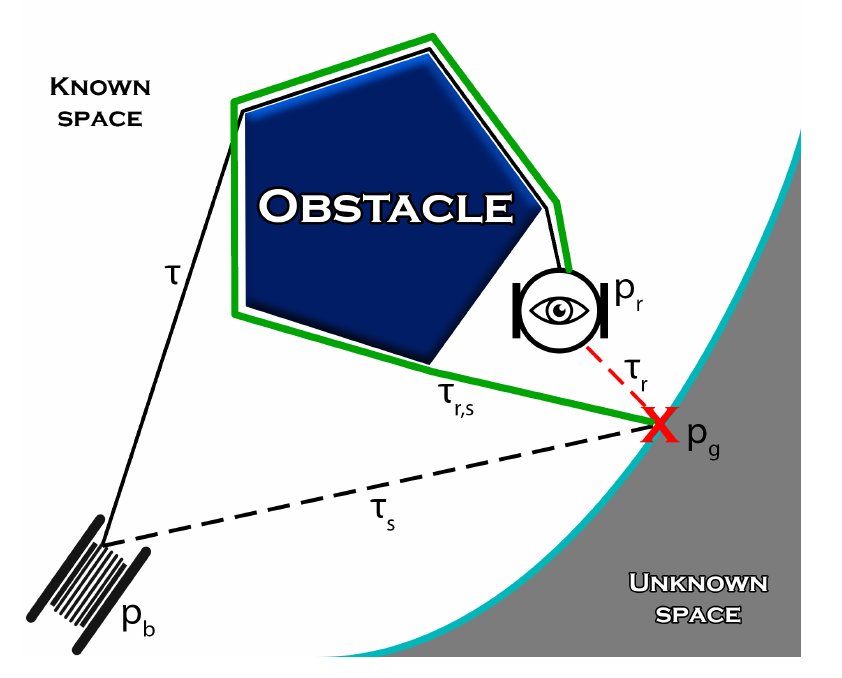
\includegraphics[scale=.3]{tethered_exploration}
  \caption{The robot at position \(p_{r}\) chooses path
    \(\tau_{r, s}\) because \(\tau + \tau_{r, s}\) is homotopic to the
    shortest path \(\tau_{s}\). Notice that \(\tau + \tau_{r}\) is not
    null-homotopic and would entangle the tether
    \cite{shapovalovExplorationUnknownEnvironments2020}.}
  \label{fig:tethered-exploration}
\end{figure}

Zhou et. al. \cite{zhouRobustRealtimeUAV2020} applied the concept of
different homotopy classes to aggresive UAV flight. They use it to
activate a more comprehensive exploration of the search space of
gradient-based trajectory optimization which is used for trajectory
replanning and is prone to getting stuck in local minima.

Orthey et. al. \cite{ortheyMotionPlanningExplorer2020} created a
visual explorer that shows different local minima given a start and
endpoint. Local minima are defined to be classes of paths that
converge to the same minimum under minimization of a chosen cost
functional.

Wu et. al. \cite{wuMultiRobotPathDeconfliction2020} propose a method
to deconflict paths of multiple robots in cluttered environments.
Sequencially each robot computes it's path. The order is determined by
the number of homology classes of paths of each robot.

A solution for a similar problem is shown by Wang
et. al. \cite{wangCoordinationfreeMultirobotPath2022}. They show a
solution to multi-robot path planning in complex cluttered
environments without inter-robot communication or coordination. The
approach assigns robots stochastically to different topological
classes and uses a potential field based controller to avoid local
obstacles.

\begin{table*}
  \centering
  \begin{tabular}{l c p{8cm}}
    \hline
    Homotopy & & \\
    \hline
    Bhattacharya
    et. al. \cite{bhattacharyaSearchbasedPathPlanning2010} & 2010 &
                                                                    2-D
                                                                    homotopy
                                                                    invariant
                                                                    based on
                                                                    Cauchy's
                                                                    Integral
                                                                    Theorem
                                                                    and
                                                                    Residue
                                                                    Theorem \\
    Bhattacharya
    et. al. \cite{bhattacharyaSearchBasedPathPlanning2012} & 2012 & 3-D
                                                                    homtopy
                                                                    invariant
                                                                    based on
                                                                    Biot-Severts
                                                                    Law and
                                                                    Ampere's
                                                                    Law \\
    Bhattacharya et. al. \cite{bhattacharyaPathHomotopyInvariants2018}
             & 2018 &
                      homotopy invariants using
                      \((D - 1)\)-dimensional
                      submanifolds and word
                      construction \\
    Sakcak et. al. \cite{sakcakHomotopyAwareKinodynamic2019} & 2019 &
                                                                      blabla
    \\
    Shapovalov
    et. al. \cite{shapovalovExplorationUnknownEnvironments2020} & 2020
               & entangle-free exploration
                 of unknown environments
                 with tethered robot \\
    Zhou et. al. \cite{zhouRobustRealtimeUAV2020} & 2020 & improve
                                                           gradient-based
                                                           trajectory
                                                           optimization
                                                           prone to
                                                           local
                                                           minima with
                                                           homtopy
                                                           classes \\
    Orthey et. al. \cite{ortheyMotionPlanningExplorer2020} & 2020 &
                                                                    visualize
                                                                    local
                                                                    minima \\
    Wu et. al. \cite{wuMultiRobotPathDeconfliction2020} & 2020 &
                                                                 deconfliction
                                                                 of
                                                                 multiple
                                                                 paths
    \\
    Liang et. al. \cite{liangHomotopyDrivenExplorationHumanmade2021} &
                                                                       2021 &
                                                                              human-made
                                                                              space
                                                                              exploration
                                                                              using
                                                                              signs
                                                                              and
                                                                              homotopy
                                                                              exploration
                                                                              strategy
    \\
    Wang et. al. \cite{wangConstructingFinerThen2022} & 2022 &
                                                               finer than
                                                               homotopy
                                                               classes \\
    Yang et. al. \cite{yangEfficientSearchShortest2022} & 2022 &
                                                                 \(k\)-shortest
                                                                 non-homotopic
                                                                 paths \\
    Wang et. al. \cite{wangCoordinationfreeMultirobotPath2022} & 2022
               & mulit-agent path planning
                 without communication and
                 coordination \\
    \hline
    Fiber Bundle & & \\
    \hline
  \end{tabular}
  \caption{Topological methods combined with the path planning
    problem.}
  \label{tab:topological-methods}
\end{table*}

\subsection*{Conclusion}
This review of topological methods in robot path planning shows that
the topological properties of the configuration space play a
fundamental role in solving the path planning problem. These
properties can be used for example in exploration, multi-robot path
planning or path optimization. We believe that making use of the
additional knowledge of the structure of the configuration space
allows for faster and more intelligent algorithms. Both of these
traits are the motivation of more than a decade of research in robot
path planning.

Possible future research directions include:
\begin{enumerate}
\item Can existing or new topological invariants be used to calculate
  admissible heuristics to speed up existing path planning algorithms
  like for example A*?
\item Can the topological properties be encoded
  \cite{chazalIntroductionTopologicalData2021} and fed into other
  machine learning models to increase their understanding and boost
  performance?
\end{enumerate}

\bibliographystyle{plain} \bibliography{../bib/mybib}

\end{document}
